\documentclass[border=5pt]{standalone}
% Style commun aux figures de structure de MPMbox
% ------------------------------------------------
\usepackage[utf8]{inputenc}
\usepackage[T1]{fontenc}
\usepackage[english]{babel}
\usepackage{lmodern}
\usepackage{tikz}
\usetikzlibrary{positioning,arrows.meta,calc,fit,backgrounds,shapes.geometric}
% babel(french) rend « : » actif, ce qui casse les coordonnées polaires (90:4cm)
\usetikzlibrary{babel}

% pas de césure dans les boîtes étroites
\hyphenpenalty=10000
\exhyphenpenalty=10000
\tolerance=9999
\emergencystretch=3em

\definecolor{mpmBase}{HTML}{1F3A5F}    % classes de base
\definecolor{mpmBaseBg}{HTML}{E8EEF6}
\definecolor{mpmDeriv}{HTML}{4A7BA7}   % variantes
\definecolor{mpmDerivBg}{HTML}{F5F8FB}
\definecolor{mpmData}{HTML}{7A5230}    % données simulées
\definecolor{mpmDataBg}{HTML}{FBF3E8}
\definecolor{mpmAccent}{HTML}{A6432F}  % mise en avant (MPMxDEM)
\definecolor{mpmAccentBg}{HTML}{FBEEEB}
\definecolor{mpmGrey}{HTML}{5A6472}

\tikzset{
  base/.style={
    draw=mpmBase, line width=0.9pt, fill=mpmBaseBg, rounded corners=3pt,
    text width=#1, align=center, inner sep=6pt, font=\sffamily\small},
  base/.default=5.2cm,
  deriv/.style={
    draw=mpmDeriv, line width=0.6pt, fill=mpmDerivBg, rounded corners=2pt,
    text width=#1, align=left, inner sep=5pt, font=\sffamily\scriptsize},
  deriv/.default=7.4cm,
  data/.style={
    draw=mpmData, line width=0.7pt, fill=mpmDataBg, rounded corners=3pt,
    text width=#1, align=center, inner sep=5pt, font=\sffamily\scriptsize},
  data/.default=4.2cm,
  accent/.style={
    draw=mpmAccent, line width=0.8pt, fill=mpmAccentBg, rounded corners=2pt,
    text width=#1, align=left, inner sep=5pt, font=\sffamily\scriptsize},
  accent/.default=7.4cm,
  spine/.style={draw=mpmDeriv, line width=0.6pt},
  link/.style={draw=mpmGrey, line width=0.6pt, -{Stealth[length=4pt]}},
  dashlink/.style={draw=mpmGrey, line width=0.6pt, densely dashed,
                   -{Stealth[length=4pt]}, font=\sffamily\tiny},
  mpmcap/.style={font=\sffamily\scriptsize\itshape, text=mpmGrey},
}

% Titre d'une classe de base : \classname{Nom}{rôle}
\newcommand{\classname}[2]{{\bfseries #1}\\[2pt]{\scriptsize\itshape #2}}
% Ligne d'une variante : \variant{Nom}{description}
\newcommand{\variant}[2]{{\bfseries\ttfamily #1}\quad #2}

\begin{document}
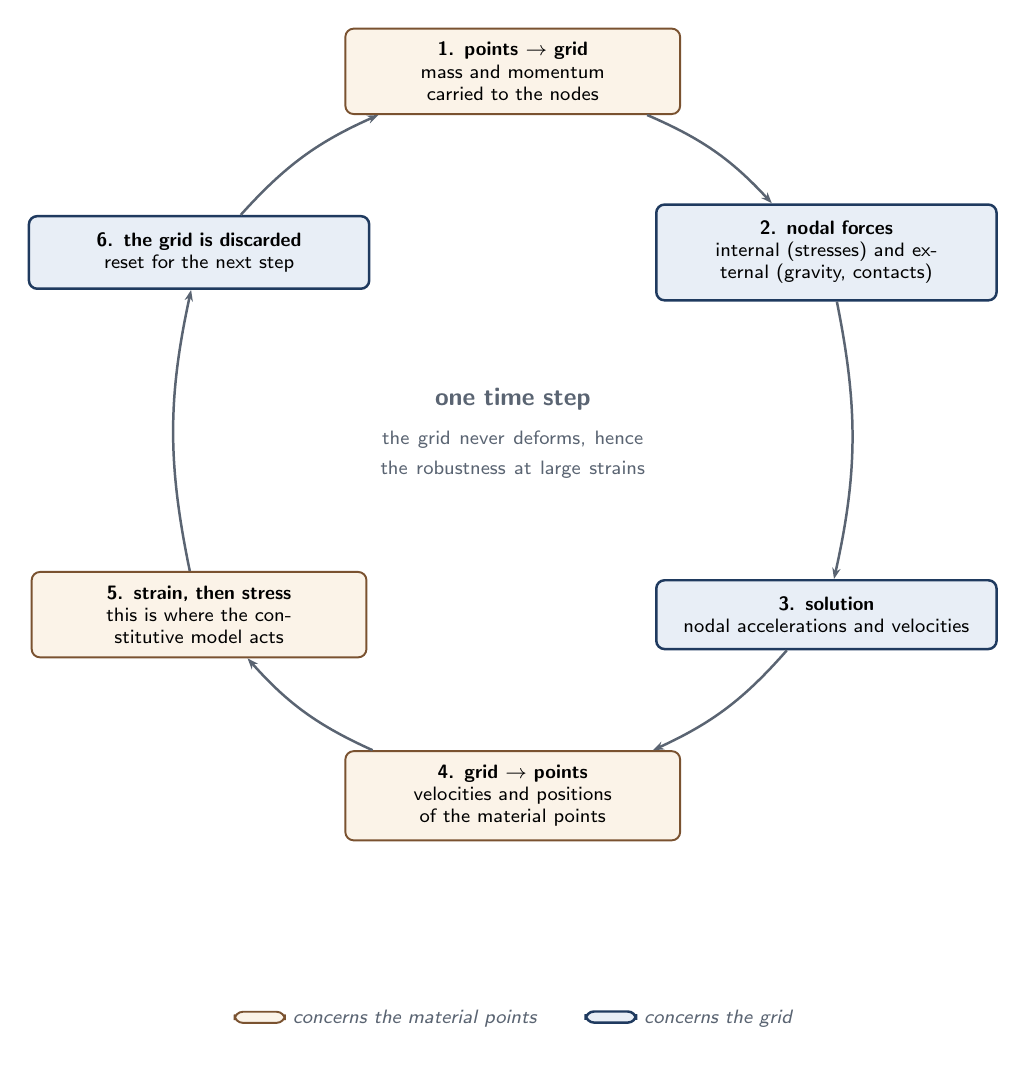
\begin{tikzpicture}

\def\R{4.6cm}

\node[data=3.9cm] (N1) at ( 90:\R) {{\bfseries 1. points $\rightarrow$ grid}\\ mass and momentum carried to the nodes};
\node[base=3.9cm, font=\sffamily\scriptsize] (N2) at ( 30:\R) {{\bfseries 2. nodal forces}\\ internal (stresses) and external (gravity, contacts)};
\node[base=3.9cm, font=\sffamily\scriptsize] (N3) at (-30:\R) {{\bfseries 3. solution}\\ nodal accelerations and velocities};
\node[data=3.9cm] (N4) at (-90:\R) {{\bfseries 4. grid $\rightarrow$ points}\\ velocities and positions of the material points};
\node[data=3.9cm] (N5) at (-150:\R) {{\bfseries 5. strain, then stress}\\ this is where the constitutive model acts};
\node[base=3.9cm, font=\sffamily\scriptsize] (N6) at ( 150:\R) {{\bfseries 6. the grid is discarded}\\ reset for the next step};

\foreach \a/\b in {1/2,2/3,3/4,4/5,5/6,6/1} {
  \draw[link, line width=0.9pt] (N\a) to[bend left=12] (N\b);
}

\node[text width=4.0cm, align=center, font=\sffamily\small, text=mpmGrey] at (0,0)
  {{\bfseries one time step}\\[3pt]
   {\scriptsize the grid never deforms, hence the robustness at large strains}};

\node[mpmcap, anchor=north, text width=11cm, align=center] at (0,-7.2)
  {\tikz\node[data=0.5cm, inner sep=2pt]{}; concerns the material points
   \qquad
   \tikz\node[base=0.5cm, inner sep=2pt]{}; concerns the grid};

\end{tikzpicture}
\end{document}
